\documentclass[12pt]{article}
\usepackage{graphicx}
\usepackage{float}
\usepackage{amsmath}
\title{Experiment 3: Prime Detector}
\author{Annirudh K P\\%
210070009}

\begin{document}

\maketitle

\section{Overview of the experiment}
\paragraph{}
In this experiment, we started working on more designs using structure modelling on VHDL. The problem statement of this experiment is to design a Prime Detector, whose function we derive using the K-Maps. The objective of this experiment was to understand the Quartus Design Flow, work with the Xen10 Board, and give us hands on experience over different technical glitches/problems we may face in this piece of software which has been made unwantedly hard.

\section{Experimental Set-up}

\subsection{Design Requirements}
\subsubsection{Prime Detector}
The Prime Detector takes in every decimal number in its binary form (4 bits). The output is a simple 0 if not prime, and 1 if it is prime.

\begin{figure}[H]
\centering
  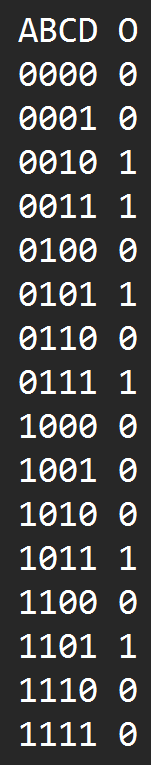
\includegraphics[scale=0.3]{Images/PrimeNumber_TT.png}
  \caption{Prime Detector Truth Table}
\end{figure}

\subsection{Design Schematics}
The following design schematics are shown. The min-function was first got from K-Map, and then the design was implemented. Also we have to design 3 input AND gates and 4 input OR gate for the same additionally. 

\begin{figure}[H]
\centering
  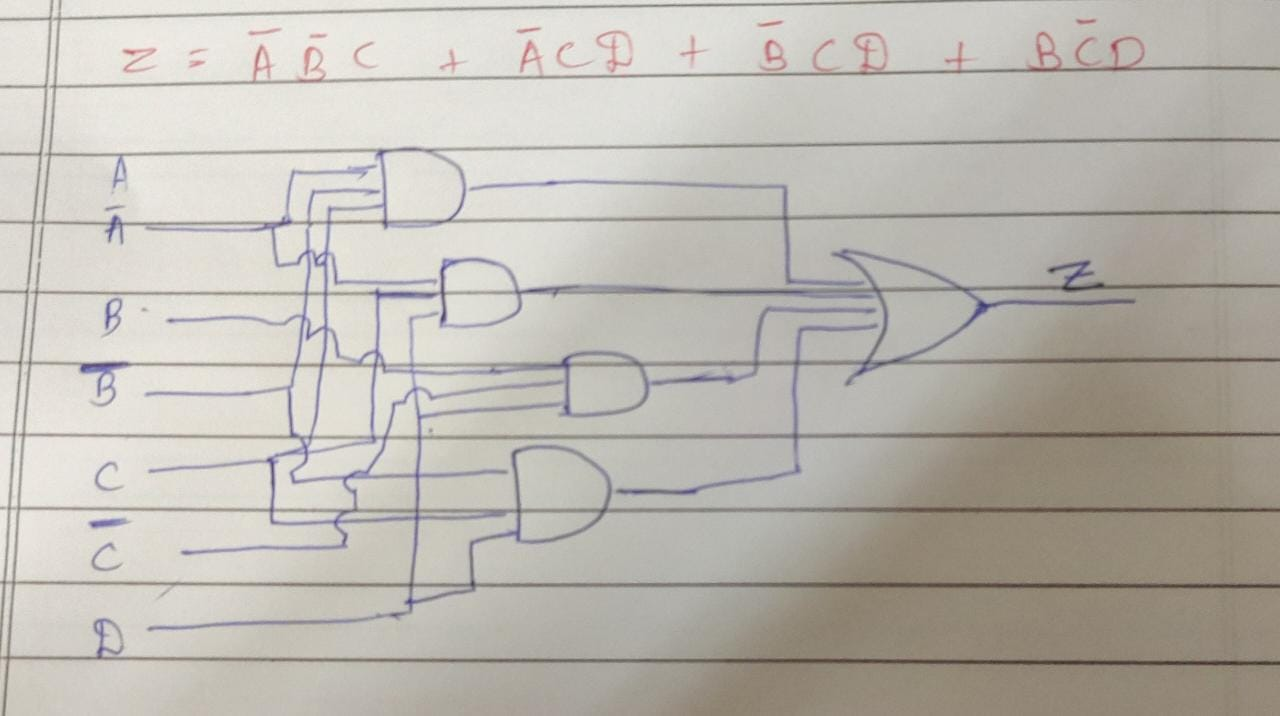
\includegraphics[scale=0.3]{Images/PrimeNumber_Design.jpeg}
  \caption{Prime Decider Design}
\end{figure}

\begin{figure}[H]
\centering
  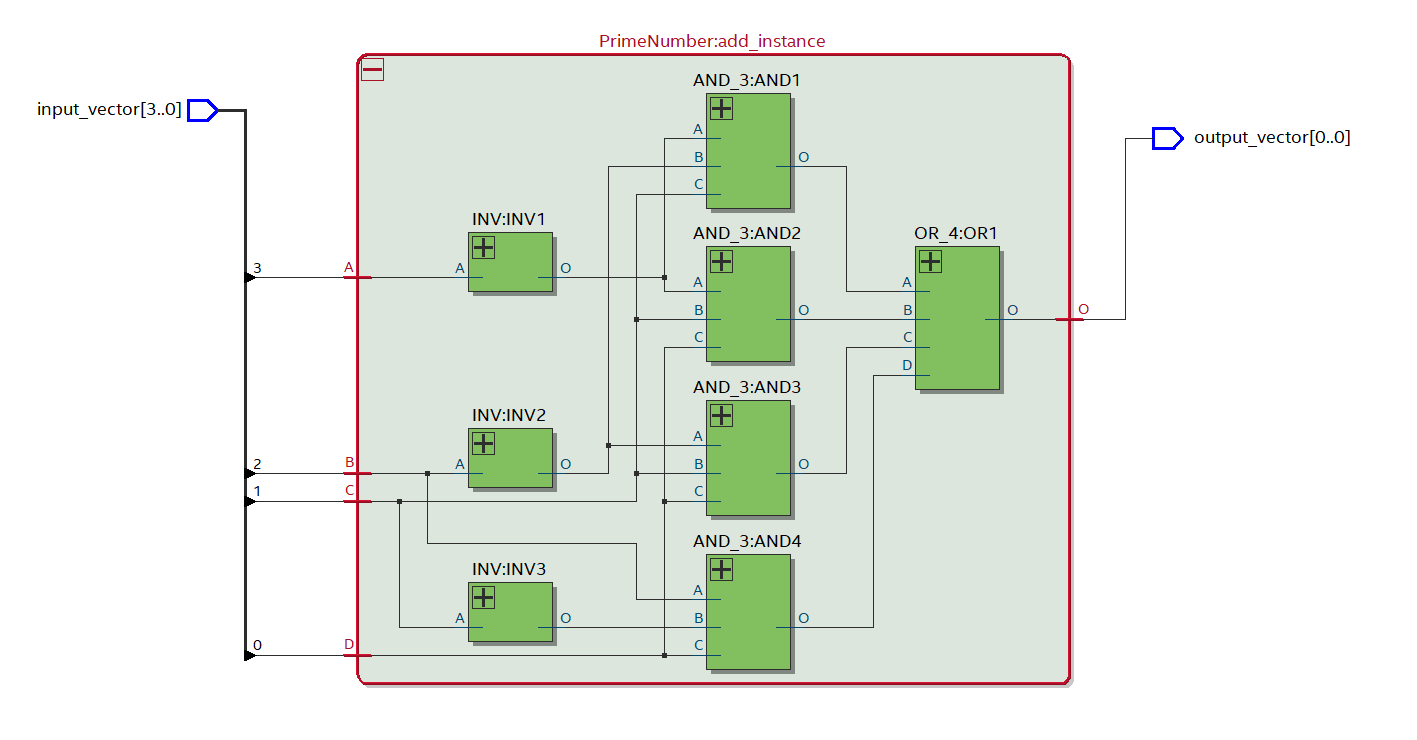
\includegraphics[scale=0.3]{Images/PrimeNumber_RTLViewer.png}
  \caption{Prime Detector RTL Design}
\end{figure}

\subsection{Description of Components}
\subsubsection{Prime Detector}
\begin{verbatim}
library ieee;
use ieee.std_logic_1164.all;

entity OR_4  is
  port (A, B, C, D: in std_logic; O: out std_logic);
end entity OR_4;

architecture Struct of OR_4 is
begin
	O <= A or B or C or D;
end Struct;

library ieee;
use ieee.std_logic_1164.all;

entity AND_3  is
  port (A, B, C: in std_logic; O: out std_logic);
end entity AND_3;

architecture Struct1 of AND_3 is
begin
	O <= A and B and C;
end Struct1;

library ieee;
use ieee.std_logic_1164.all;

entity INV  is
  port (A: in std_logic; O: out std_logic);
end entity INV;

architecture Struct3 of INV is
begin
	O <= not(A);
end Struct3;

library ieee;
use ieee.std_logic_1164.all;

entity PrimeNumber  is
  port (A, B, C, D: in std_logic; O: out std_logic);
end entity PrimeNumber;

architecture Struct2 of PrimeNumber is
	signal S1, S2, S3, S4, A_b, B_b, C_b : std_logic;
	component OR_4 is
		port (A, B, C, D: in std_logic; O: out std_logic);
	end component OR_4;
	component AND_3 is
		port (A, B, C: in std_logic; O: out std_logic);
	end component AND_3;
	component INV is
		port (A: in std_logic; O: out std_logic);
	end component INV;
begin
	INV1:	INV port map (A => A, O => A_b);
	INV2:	INV port map (A => B, O => B_b);
	INV3:	INV port map (A => C, O => C_b);
	AND1: AND_3 port map (A => A_b, B => B_b, C => C, O => S1);
	AND2: AND_3 port map (A => A_b, B => C, C => D, O => S2);
	AND3: AND_3 port map (A => B_b, B => C, C => D, O => S3);
	AND4: AND_3 port map (A => B, B => C_b, C => D, O => S4);
	OR1: OR_4 port map (A => S1, B => S2, C => S3, D => S4, O => O);
end Struct2;
\end{verbatim}

\section{Observations}
 
We get RTL simulation waveforms for corresponding to input and output which is given below and it shows required results.

\begin{figure}[H]
\centering
  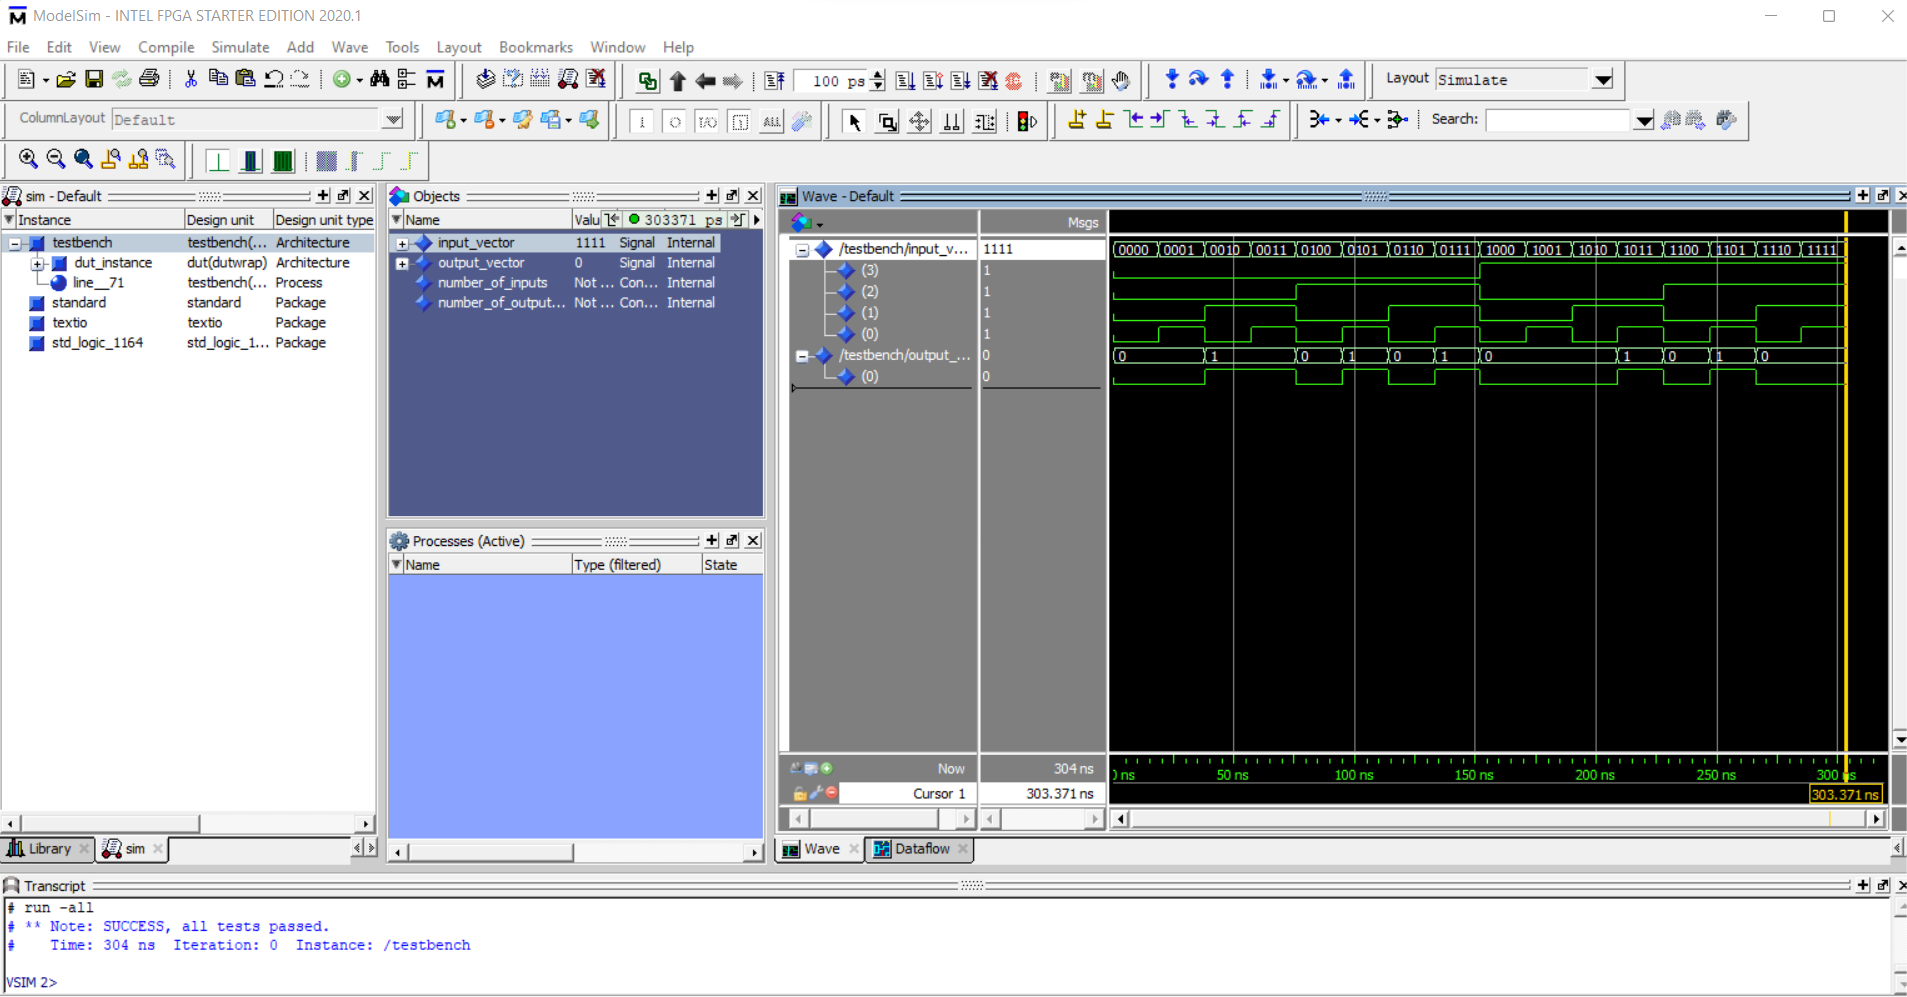
\includegraphics[scale=0.35]{Images/PrimeNumber_RTLSimulation.png}
  \caption{Prime Detector RTL Simulation Waveform}
\end{figure}

Further the code (in form of .svf file) was flashed onto the Xen10 board, after the pins and LED were mapped accordingly. The output verified the working of the logic, and some example images are shown below.

\begin{figure}[H]
\centering
  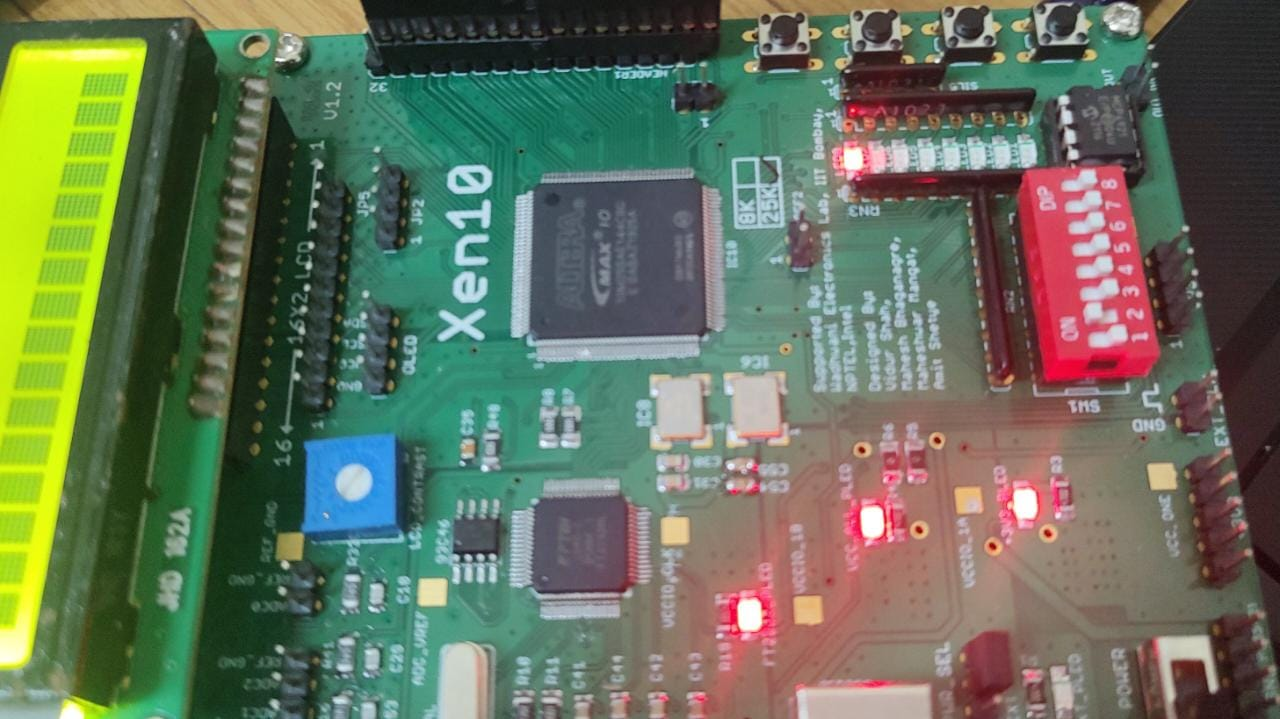
\includegraphics[scale=0.35]{Images/Trial01.jpeg}
  \caption{Prime Detector Example 1 - Xen10 Board}
\end{figure}

\begin{figure}[H]
\centering
  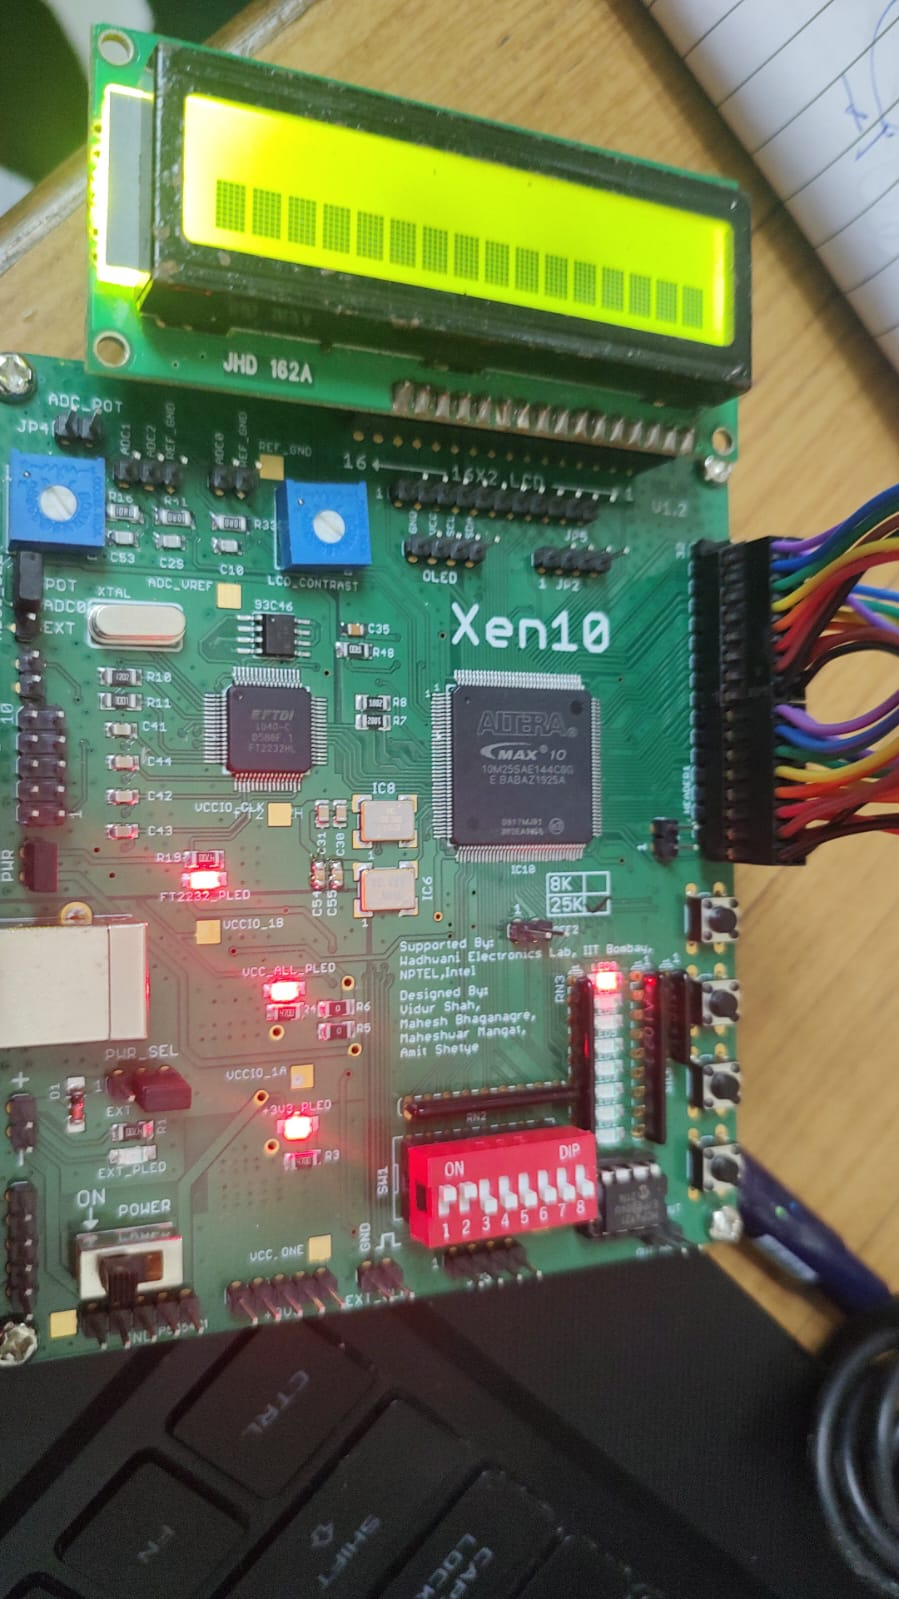
\includegraphics[scale=0.35]{Images/Trial02.jpeg}
  \caption{Prime Detector Example 2 - Xen10 Board}
\end{figure}

\begin{figure}[H]
\centering
  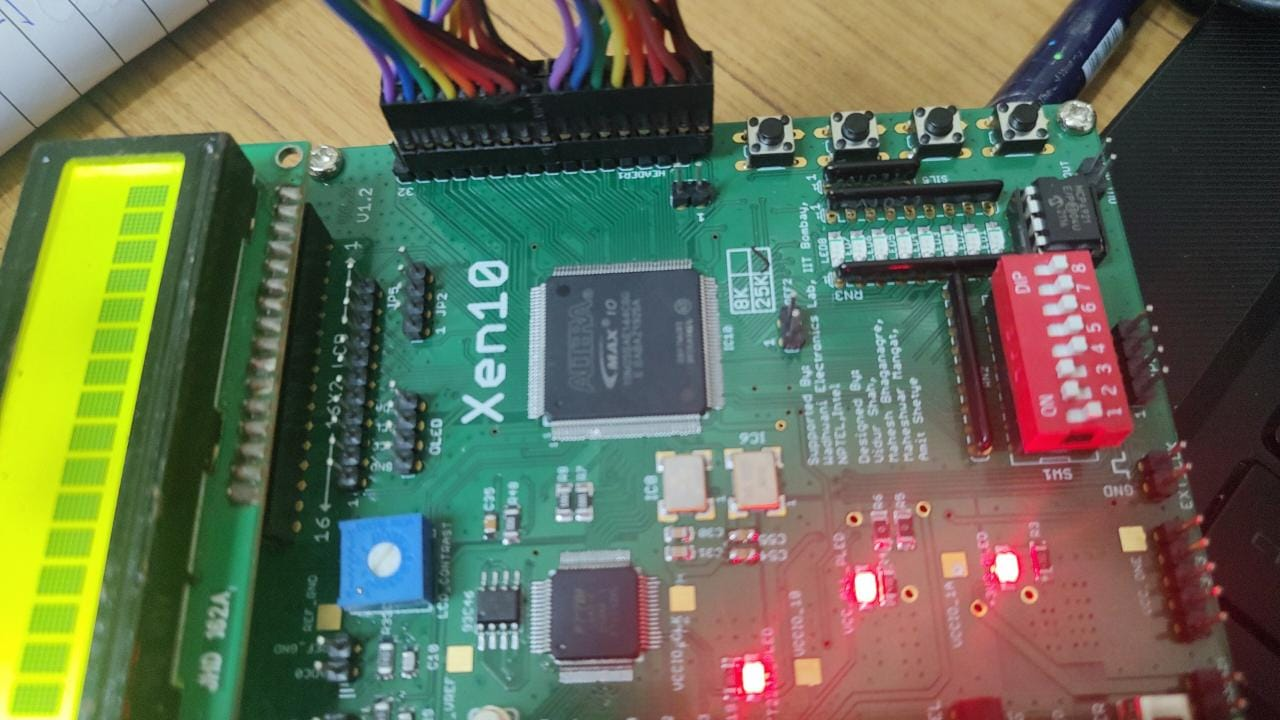
\includegraphics[scale=0.35]{Images/Trial03.jpeg}
  \caption{Prime Detector Example 3 - Xen10 Board}
\end{figure}

\end{document}